\documentclass{article}
\usepackage{amsmath}
\usepackage{amssymb}
\usepackage{hyperref}
\usepackage{graphicx} % Required for inserting images
\usepackage{soul}
\usepackage[]{geometry}

\title{\textbf{Project Report}\\[0.5em] \Large \textbf{Approximate Distance Oracles: A Randomized Approach}}
\author{
    \vspace{0.5cm} \\
    \textbf{Submitted by:} \\[0.5em]
    Kartik Anant Kulkarni (210493) \\ 
    Siddharth Garg (211031) \\ 
    Goural Dureja (210393) \\[1.5em]
    \textbf{Under the Guidance of:} \\[0.5em]
    Prof. Surender Baswana \\[1.5em]
    \textbf{CS648: Randomized Algorithms} \\ 
    Indian Institute of Technology, Kanpur
}


\date{11th April, 2025}

\begin{document}

\maketitle

\vspace{1cm}

\section*{Acknowledgment}

We are extremely grateful to our professor, Prof. Surender Baswana, for his unwavering support, expert guidance, and invaluable suggestions throughout the project. His insights played a key role in refining our approach and in the development of our algorithms. In particular, the hints provided during discussions about 3-approximate distance oracles and advice on extending these ideas to a 5-approximate variant were crucial in enabling us to generalize the method to a \((2k-1)\)-approximate oracle. We would also like to emphasize that, aside from some initial background reading on implementation techniques, no external assistance was used in the development of this project. Overall, this experience has been highly educational, offering us a practical insight into the challenges and problem-solving required in algorithm design and evaluation—mirroring the real-world complexities faced by researchers in the field.

\newpage

\tableofcontents

\newpage

\section{Problem Statement}
The aim of this project is to build a space-efficient approximate distance oracle for a non-negative weighted undirected graph \(G=(V,E)\) that returns a \((2k-1)\)-approximation of the true distance between any two vertices in just \(O(k)\) time. The algorithm developed would be practically experimentally on real-world datasets to validate the theoretical results and observe the impact of randomized algorithms in the real-world. 

\section{Introduction}

Consider an undirected non-negative weighted graph \(G = (V, E)\) with \(n = |V|\) vertices and \(m = |E|\) edges. The stretch of a distance oracle is defined as the ratio of the approximate distance reported by the oracle to the true shortest path distance. Mathematically, for any two vertices \(u\) and \(v\), the stretch is given by:

\[
\text{Stretch}(u, v) = \frac{d_{\text{approx}}(u, v)}{\delta(u, v)},
\]

where \(d_{\text{approx}}(u, v)\) is the approximate distance returned by the oracle, and \(\delta(u, v)\) is the true shortest path distance between \(u\) and \(v\) {as reported by the All-Pairs Shortest Paths Problem (APSP)}. Our goal is to answer queries with a maximum stretch of \(2k - 1\) for any two vertices in \(O(k)\) time.

Our approach constructs a distance oracle in \(O\Bigl(k \, m \, n^{1/k}\Bigr)\) expected time. The oracle occupies \(O\bigl(k\,n^{1+1/k}\bigr)\) expected space (in the word RAM model) and can answer any \((2k-1)\)-approximate distance query in constant \(O(k)\) time. We also construct a space efficent version of the algorithm that would further give us a worst case \(O\bigl(k\,n^{1+1/k}\bigr)\) space. The key idea behind our approach is to trade exactness for efficiency by carefully selecting and storing only a subset of the distance information.

Finally, we implement the algorithm in C++ and analyse the performance on different real-world graphs for various conditions.

\section{Initial Deterministic Attempts}

Before exploring the randomized approach for selecting landmark vertices, we considered if we can solve the challenge deterministic strategies. Both methods, however, face significant challenges in balancing the number of landmarks with the resulting ball sizes.

\subsection{Method 1: Vertex-Specific Landmark Selection}

One idea was to assign each vertex \(w\) to a landmark \(u \in L\) such that the ball \(\text{Ball}(u)\) remains as small as possible (e.g., by performing a breadth-first search and selecting the next closest vertex). Although this keeps the ball sizes small, it tends to produce a large number of landmarks:
\begin{itemize}
    \item \textbf{Advantage:} Restricting each ball to a tightly bounded size.
    \item \textbf{Drawback:} In the worst case, there is minimal or no sharing of landmarks among different vertices. Consequently, the landmark set \(L\) could become very large, and its size is highly graph-dependent. 
\end{itemize}

\subsection{Method 2: Regular Spacing by Sorted Distances}
Another attempt was to fix an initial landmark vertex (e.g., a root or ``0th node''), compute distances for all other vertices, sort them by distance, and then designate every \(\sqrt{n}\)th vertex in the sorted list as a landmark:
\begin{itemize}
    \item \textbf{Advantage:} The number of landmarks can be predetermined, offering a fixed cap.
    \item \textbf{Drawback:} Estimating the ball sizes for each landmark becomes difficult. Cross-connections and variations in the underlying graph may cause excessive aggregation in some balls.
\end{itemize}

\subsection{Trade-Off and Move to Randomization}
Both of these deterministic techniques highlight a tension between the number of landmark points (\( |L| \)) and the size of the balls \(\text{Ball}(u)\). Overly restrictive strategy on ball size risk exploding the landmark set, while methods ensuring a fixed landmark count can produce unmanageably large balls. This trade-off motivates the use of a \emph{randomized} method, which, in expectation, balances the size of each ball and the total number of landmarks more effectively. Consequently, the randomized approach offers a tunable and provably efficient compromise between these competing objectives. In the following section, we describe one such instantiation: the 3-Approximate Distance Oracle, which demonstrates how approximate distances can be obtained with minimal overhead.

\section{3-Approximate Distance Oracle}
To improve efficiency over maintaining full APSP data, we sacrifice exactness by approximating distances. Instead of storing the exact distance between every pair of vertices, each vertex keeps distances only to a limited subset of other vertices. Moreover, for a carefully selected group of vertices—referred to as \emph{landmark vertices}—we compute and store the distances from these landmarks to all vertices in the graph. This design enables fast query responses while ensuring that the approximated distances are within a factor of 3 of the true shortest path lengths.

\subsection{Algorithm Overview}
The oracle is built using a two steps:
\begin{itemize}
    \item \textbf{Landmark Vertices:} A set of landmark vertices is chosen by sampling vertices with probability of a particular vertex being landmark point as \textit{p}. For each landmark point, the shortest path distance to every other vertex is computed.
    \item \textbf{Selective Storage:} For each vertex, only a small subset of distances to nearby vertices (which are closer than the nearest landmark point) is stored. This significantly reduces the storage overhead compared to storing all pairwise distances.
\end{itemize}
\subsection{Query Processing}
When a query is made for the distance between two vertices \(u\) and \(v\), the oracle proceeds as follows:

\begin{enumerate}
    \item \textbf{Direct Distance Available:}  
    If the oracle has stored the direct distance between \(u\) and \(v\) — typically when they lie within each other’s local vicinity — it returns this distance immediately without further computation.
    \newline
    \item \textbf{Indirect Distance via Landmark:}  
    If the direct distance is not stored, the oracle uses \textit{l(u)} or \textit{l(v)} which is the nearest landmark point to vertex \textit{u} and \textit{v} respectively. In this scenario, the approximate distance is computed as:
    \[
    d_{\text{approx}}(u,v) = \delta(u,l) + \delta(l,v),
    \]
    where \(\delta(u,l)\) and \(\delta(l,v)\) are the precomputed distances from \(u\) to \(l\) and from \(l\) to \(v\) respectively. This approximation is guaranteed to be within a factor of 3 of the true shortest path length.
\end{enumerate}

\subsection{Proof of Correctness}
We now prove that for any two vertices \(u\) and \(v\) in \(G\), there exists a landmark \(l\) such that the approximate distance

\[
d_{\text{approx}}(u,v) = \delta(u,l) + \delta(l,v), \quad \text{satisfies} \quad d_{\text{approx}}(u,v) \le 3\,\delta(u,v).
\]

\paragraph{Proof:} 

\noindent For each vertex \(x \in \{u,v\}\), let \(l(x)\) denote the landmark vertex closest to \(x\); that is,
\[
l(x) = \arg\min_{l \in L} \delta(x,l).
\]

\noindent By definition, we then have:
\(
\quad \delta(x, l(x)) \le \delta(x, y) \quad \text{for all } y \in L.
\)

\noindent Thus, we now consider two cases:

\begin{itemize}
    \item \textbf{Case 1}: \(l(u) = l(v)\).  
    If both \(u\) and \(v\) share the same closest landmark, say \(l = l(u) = l(v)\), then we can apply the triangle inequality (which is simply, a result of the definition of the shortest distance \(\delta\)),
    \[
    \delta(u,v) \le \delta(u,l) + \delta(l,v).
    \]
    
    Moreover, since \(l\) is the closest landmark for both \(u\) and \(v\), it follows that
    \[
    \delta(u,l) \le \delta(u,v) \quad \text{and} \quad \delta(l,v) \le \delta(u,v).
    \]
    
    Thus,
    \(
    d_{\text{approx}}(u,v) = \delta(u,l) + \delta(l,v) \le \delta(u,v) + \delta(u,v) = 2\delta(u,v),
    \) 
    which is clearly within the desired factor of 3.
    
    \item \textbf{Case 2}: \(l(u) \neq l(v)\).
    In this case, we choose one of the landmarks; without loss of generality, let \(l = l(u)\). By the triangle inequality,
    \[
    \delta(l(u),v) \le \delta(l(u),u) + \delta(u,v) = \delta(u,l(u)) + \delta(u,v).
    \]
    
    Hence, the approximate distance when using \(l(u)\) is given by,
    \[
    d_{\text{approx}}(u,v) = \delta(u,l(u)) + \delta(l(u),v) \le \delta(u,l(u)) + \bigl(\delta(u,l(u)) + \delta(u,v)\bigr) = 2\delta(u,l(u)) + \delta(u,v).
    \]
    
    Since \(l(u)\) is the closest landmark to \(u\), we have
    \(
    \delta(u,l(u)) \le \delta(u,v).
    \)
    
    Substituting this bound yields
    \(
    d_{\text{approx}}(u,v) \le 2\delta(u,v) + \delta(u,v) = 3\delta(u,v).
    \)
\end{itemize}

\noindent In both cases, we have shown that
\(
d_{\text{approx}}(u,v) \le 3\delta(u,v).
\)
Thus, the distance oracle indeed provides a 3-approximation of the true shortest path distance, completing the proof of correctness.
\hfill \(\Box\)

\subsection{Pre-processing}
During pre-processing we need to build necessary data structures for efficient query answering while reducing both computational and storage costs. This phase is divided into three key steps:

\begin{enumerate}
    \item \textbf{Landmark Selection:}  
    A subset \(L \subseteq V\) of vertices is chosen to serve as landmark vertices. This selection is performed in a randomized manner: each vertex is independently chosen as a landmark with probability \(p = \frac{1}{\sqrt{n}}\). This randomized selection ensures that, in expectation, the number of landmarks is \(O(\sqrt{n})\), providing good coverage of the graph while keeping the landmark set small.
    
     \item \textbf{Ball Construction, Local Distance Computation, and Hash Table Setup:}  
    For every vertex \(u \in V\), let \(l(u)\) denote the landmark vertex closest to \(u\). We then define the \emph{ball} of \(u\) as
    \[
    B(u) = \{ v \in V \mid \delta(u,v) < \delta(u, l(u)) \}.
    \]
    This set comprises all vertices that are closer to \(u\) than its nearest landmark. Within this ball, the exact distance \(d(u,v)\) for all \(v \in B(u)\) are computed and stored. To achieve \textit{O(1)} time distance lookups, for each vertex \(u\) we will create a hash table to store \textit{Ball(u)}. The size of each hash table is proportional to the size of its respective ball.
    
    \item \textbf{Distance Computation for Landmarks:}  
    To compute the shortest distance for each landmark point to all vertices, we use multi-source Dijkstra, which is equivalent to adding a dummy node, connected to all landmarks by a 0 weighted edge, and this dummy node is chosen as the source. These global distances from each landmark allow the oracle to efficiently approximate the distance between vertices that are not within each other's balls.
\end{enumerate}

\noindent \textit{Note:} Here, we are missing a method of efficiently computing a ball for every vertex as the naive Dijkstra algorithm will not achieve the required time complexity. The modification in Dijkstra is described later to achieve the required bound.

\subsection{Complexity Analysis for the 3-Approximate Distance Oracle}
\paragraph{Space Complexity:}  
To analyze the space required by the 3-approximate distance oracle, we consider the storage needed for each vertex \(u \in V\). Let the vertices of \(V \setminus \{u\}\) be ordered as \(\{v_1,v_2,\ldots,v_{n-1}\}\) in non-decreasing order of their distance from \(u\). Define the set \(Ball(u)\) as those vertices in \(V\setminus\{u\}\) that are closer to \(u\) than the nearest vertex in a randomly sampled set \(L\). In this scheme, each vertex is chosen independently to be part of \(L\) with probability \(p\), and here we take \(p=1/\sqrt{n}\).

A vertex \(v_i\) will belong to \(Ball(u)\) if none of the vertices \(v_1, v_2, \dots, v_{i-1}\) have been selected into \(L\). Thus, the probability that \(v_i\) is in \(S_u\) = \((1-p)^{i-1}.\)
By linearity of expectation, the expected size of \(Ball(u)\) is
\[
\mathbb{E}[|S_u|] = \sum_{i=1}^{n-1} (1-p)^{i-1} \le \frac{1}{p}.
\]
In other words, on average, each vertex \(u\) stores distances to no more than \(1/p\) vertices in its set \(S_u\).

In addition to the \(S_u\) sets, the landmark vertices are used to store distances to all other vertices, and this contributes an extra \(O(n^2 p)\) term to the space. Thus, the total expected space required by the oracle is given by:
\(
O\left(n^2p + \frac{n}{p}\right).
\)
Choosing \(p = \frac{1}{\sqrt{n}}\) minimizes the total storage, yielding an overall expected space complexity of
\(
O\left(n^{3/2}\right).
\)

\paragraph{Time Complexity Analysis for the 3-Approximate Distance Oracle}

% ..............

The overall preprocessing time can be divided into two main components: processing the local distance information for each vertex and computing global distances from the landmark vertices. In our scheme, every vertex is independently selected as a landmark with probability \(p=\frac{1}{\sqrt{n}}\).

For each vertex \(u\), the local distance processing involves building a set \(Ball(u)\) consisting of vertices that are closer to \(u\) than its nearest landmark. The expected size of \(Ball(u)\) turns out to be approximately \(1/p = \sqrt{n}\), leading to an overall local processing time of \(O(n^{3/2})\) when summed over all vertices.

In addition, since the expected number of landmarks is \(\sqrt{n}\), running a single-source shortest path algorithm from each landmark incurs an aggregate cost of \(O\Bigl(\sqrt{n}(m + n\log n)\Bigr)\).

Thus, combining both components, the total expected preprocessing time is
\[
O\Bigl(n^{3/2} + \sqrt{n}(m + n\log n)\Bigr).
\]
A detailed proof of these bounds, along with a more comprehensive analysis for the general \(k\)-approximate distance oracle, is provided in a later section.


\paragraph{Overall Preprocessing Time:}  
Combining the work done in local processing and the landmark computations, the total expected preprocessing time is
\[
O\Bigl(n^{3/2} + \sqrt{n}(m + n \log n)\Bigr).
\]
This overall time complexity reflects the efficiency gain from not computing full all-pairs shortest paths, while still ensuring that the oracle can later answer queries rapidly.


\paragraph{Query Time:} Querying the oracle involves either directly retrieving a stored local distance, if available, or combining the distances from \(u\) to a landmark and from the landmark to \(v\). Since the hashing 
used allows \textit{O(1)} lookups, the query time for a 3-approximate distance oracle is \(O(1)\).

\subsection{Space Optimized Variant of the 3-Approximate Distance Oracle}

A simple modification can transform the randomized preprocessing for the 3-approximate distance oracle into a \emph{space optimised} algorithm, which ensures correctness while maintaining expected polynomial running time and an upper bound on space utilized for storing landmark points and balls. The space utilization is pre-dominated by the balls.

An important point here is that the space utilization may blow up even if some ball gets too large although many balls are of small size. Thus, it is more meaningful to consider sum of ball size for all vertex instead of individual ball sizes. A check can be used to check that the sum of ball sizes is within a bound and repeat the pre-processing only if the size exceeds a threshold.

\paragraph{Bounding the Total Size.}
Consider all the ``balls’’ stored in the data structure. Let \(X_u\) be the size of the ball associated with vertex \(u\), and let \(
X \;=\; \sum_{u \in V} X_u \) denote sum of ball size for all vertex u.\\
By linearity of expectation: \\\(\mathbb{E}[X] = \sum_{u \in V} \mathbb{E}[X_u] = n\sqrt{n}\). \\
Markov’s Inequality states that for any constant \(c > 0\),
\[
\Pr\bigl(X \,\ge\, c\,\mathbb{E}[X]\bigr) \;\le\; \frac{1}{c}.
\]
Hence, with probability at least \(\!\!1 - \frac{1}{c}\), the total size \(X\) is at most \(c\,\mathbb{E}[X]\).

\paragraph{Algorithm.}
Using this fact, we obtain a space optimized variant of preprocessing:
\begin{enumerate}
    \item \textbf{Run the preprocessing step once}: Construct the 3-approximate distance oracle data structure in \(
O\Bigl(m \cdot n^{1/2}\Bigr).
\) time as before.
    \item \textbf{Check the data structure size}: If the total number of stored pairs \(\ensuremath{X}\) \(>\) \(c\,\ensuremath{\mathbb{E}[X]}\), \emph{discard} the structure and repeat from Step 1. Otherwise, \emph{accept} the structure and terminate.
\end{enumerate}

\paragraph{Analysis.}
By Markov’s Inequality, the probability that the constructed structure is of acceptable size in any given run is at least \(1 - \frac{1}{c}\). Thus, the expected number of runs until acceptance is
\[
\frac{1}{1 - \frac{1}{c}} \;=\; \frac{c}{c-1}.
\]
Consequently, the overall expected preprocessing time is
\(
O\!\Bigl(\tfrac{c}{c-1}\Bigr) \,\times\, 
O\Bigl(m \cdot n^{1/2}\Bigr). \;=\; \, 
O\Bigl(m \cdot n^{1/2}\Bigr). \,
\)
since \(c\) is a constant. This ensures that we achieve a guaranteed bound on the size of the data structure, while preserving the same \(
O\Bigl(m \cdot n^{1/2}\Bigr).
\) expected pre-processing time.

\section{5-Approximate Distance Oracle}
The aim here is to generalize the idea of 3-approximate distance oracle to get an oracle of smaller size with a trade-off of getting a higher stretch. More precisely, we aim to get a oracle of \(O(m \cdot n^{1/3})\) space which returns distance between two vertices (\textit{u}, \textit{v}) such that \(\delta(u, v) \leq d(u, v) \leq 5 \cdot \delta(u, v)\). 

\subsection{Construction of the Oracle}

\subsubsection{Initial Attempt}

An intuitive generalization of an approximate distance oracle from stretch $3$ to $5$ arises from attempting to extend the query procedure ``step by step'' through intermediate nodes. In the $k=2$ case (stretch $3$), the query path between two nodes $u$ and $v$ involves a single nearest landmark node (called as the focus) at level $1$, leading to a path of the form:
\[
d(u, f_1(u)) + d(f_1(u), v),
\]
with stretch at most $3$ if $v \in B_1(u)$.

When extending to $k=3$ (stretch $5$), if we store \(Ball(u, v, L_1)\), as the distances of all vertices in \(V\) from \(u\) upto closest \(L_1(u)\), called as the \emph{focus} of u, and \(Ball(l_1, V, L_2)\), as the distances of all vertices in \(V\) from \(L_1\) upto closest \(L_2(l_1)\), then we can try to proceed (See also: Figure~\ref{fig:wrongstretch}) in two steps in the worst-case (when v is not in both balls):
\[
d(u, L_1(u)) + d(L_1(u), L_2(L_1(u))) + d(L_2(L_1(u)), v),
\]

However, it is easy to see that, following earlier derivations of the triangle inequality, if the balls are constructed accordingly, then each segment in the path may individually incur a stretch up to $3$, compounding to an overall stretch of $7$. The core reason of the mistake is assuming that local triangle inequalities and greedy shortcuts preserve the global stretch bound. Losing our reference of \(u\) while querying is leading us to to overapproximation and failure to guarantee the intended stretch of $2k - 1$.

\begin{figure}
    \begin{center}
        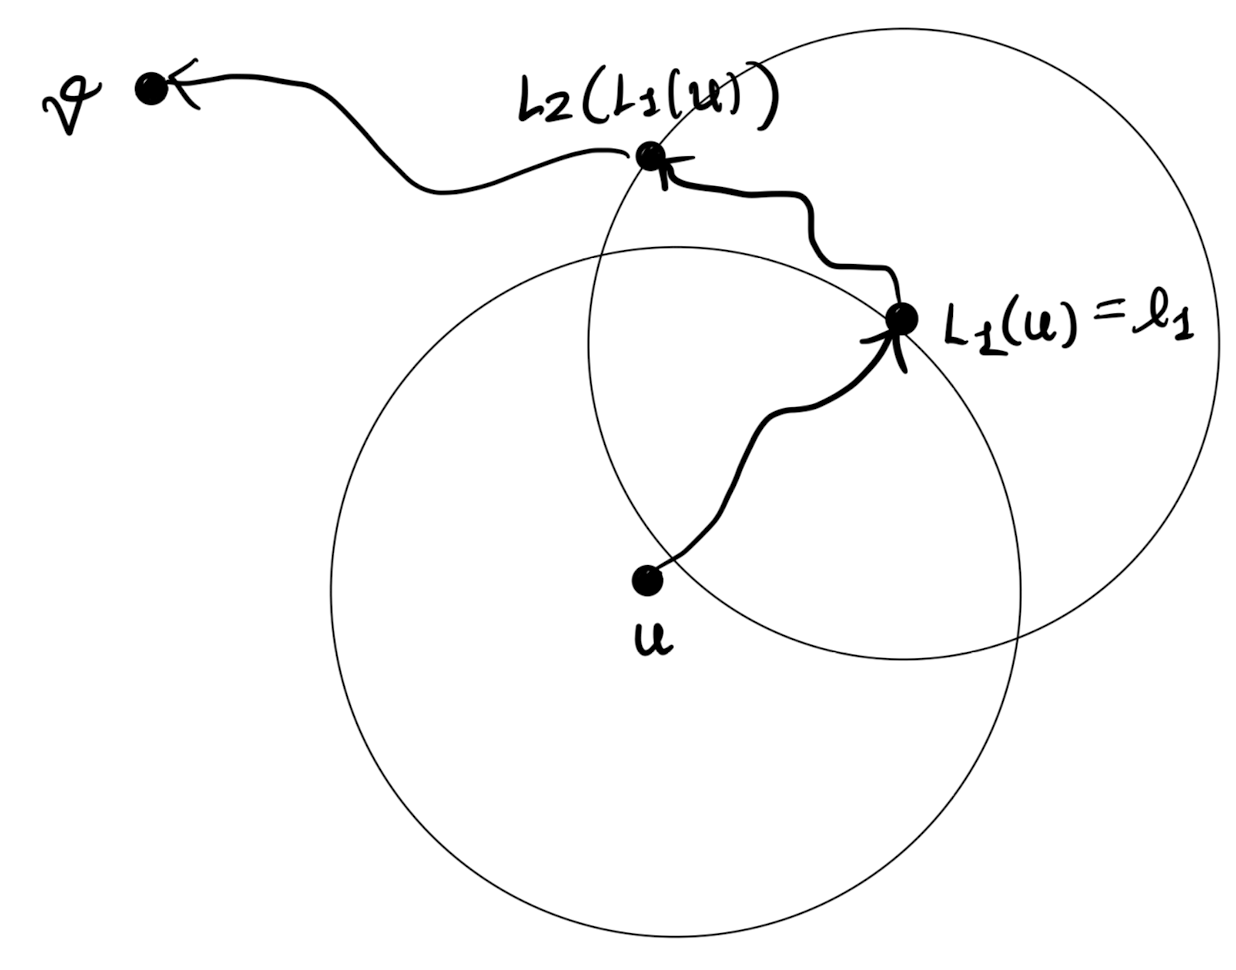
\includegraphics[width=0.4\textwidth]{img/wrongstretch.png}
        \caption{Wrong-Stretch while generalising to 5-Approximate Distance Oracle}
        \label{fig:wrongstretch}
    \end{center}
\end{figure}

\subsubsection{Improved Version}

We would like to maintain the information of u and v all way along the computation of the distance between the two vertices. Thus, a better idea would be two to store 2 balls for every vertex (instead of earlier solution), storing vertices part of $L_1$ and $L_2$ respectively. This will loosen the bound on \(\delta(u, l)\) as compared to \(\delta(u, l) \leq \delta(u, v)\) for a far away point. Further, the last level's closest landmark vertex (called as the focus), would then store the distance to all vertices. Now the distance computation between the two vertices must take place in the form of finding closest common landmark vertex between the two, so that we wouldn't have to go to the outermost level.

\subsection{Pre-processing}
\begin{enumerate}
    \item From set \textit{V} of vertices, choose each vertex to be the landmark of first level \(L_1\) with probability \(p_1 = 1/n^{1/3}\) independent of other vertices.
    \item From set \(L_1\), choose each vertex to be the landmark of second level \(L_2\) with probability \(p_2 = 1/n^{1/3}\) independent of other vertices.
    \item For each vertex \textit{u}, compute \(Ball_1(u)\) comprising vertices from \textit{V} such that \(\delta(u, v) \leq \delta(u, L_1(u))\) where \(L_1(u)\) is the vertex nearest to \textit{u} from set \(L_1\). 
    \item For each vertex \textit{u}, compute \(Ball_2(u)\) comprising vertices from \(L_1\) such that \(\delta(u, v) \leq \delta(u, L_2(u))\) where \(L_2(u)\) is the vertex nearest to \textit{u} from set \(L_2\).
    \item For each vertex \textit{u} from set \(L_2\), compute distance to all vertices of graph.  
\end{enumerate}

\noindent \textit{Note:} Again, here, we are missing a method of efficiently computing a ball for every vertex. The modification in Dijkstra is described later to achieve the required bound.

\subsection{Query Processing}
To find the distance between two vertices \textit{(u, v)}, we exploit symmetry in sense that we try to find \textit{u} in ball of vertex \textit{v} and \textit{v} in ball of vertex \textit{u}. We use the following method using conditional conditions from top to bottom for query processing: 
\begin{enumerate}
    \item If \(u \in Ball_1(v) \; : \; \text{report } \delta(u, v)\)
    \item If \(v \in Ball_1(u) \; : \; \text{report } \delta(u, v)\)
    \item If \(L_1(u) \in Ball_2(v) \; : \; \text{report } \delta(u, L_1(u)) + \delta(L_1(u), v)\)
    \item If \(L_1(v) \in Ball_2(u) \; : \; \text{report } \delta(u, L_1(v)) + \delta(L_1(v), v)\)
    \item Else \(\text{report } \delta(u, L_2(u)) + \delta(L_2(u), v)\)
\end{enumerate}
\subsection{Proof of Correctness}
Refer Figure~\ref{fig:correctstretch}. Case 1 and 2 of query processing reports the exact distance, which is within the bound.
\begin{itemize}
    \item \textbf{Case 3:} \(\delta(u, L_1(u)) \leq \delta(u, v) + \delta(v, L_1(u))\quad \text{ [Triangle Inequality]}\\
    \delta(v, L_1(u)) \leq \delta(u, v) \quad \text{\{case \textcircled{3} $\Rightarrow$ case \textcircled{2} does not hold\}} \\
    Thus,  \delta(u, L_1(v)) \leq 2\delta(u, v) \\
    \text{and} \quad \delta(u, L_1(v)) + \delta(L_1(v), v) \leq 3\delta(u, v)\) \\
    Similar analysis hold for Case 4. 
    \item \textbf{Case 5:} 
\begin{itemize}
    \item Case 1 does not hold : $\delta(u,v) \geq \delta(u, L_1(u))$
    \item Case 2 does not hold : $\delta(u,v) \geq \delta(v, L_1(v))$
    \item Case 3 does not hold : $\delta(v, L_1(u)) \geq \delta(v, L_2(v))$
    \item Case 4 does not hold : $\delta(u, L_1(v)) \geq \delta(u, L_2(u))$
\end{itemize}

Combining,\[
\delta(u, L_2(u)) + \delta(L_2(u), v) 
\leq \delta(u, L_1(v)) + \delta(L_2(u), u) + \delta(u, v) \] 
\[\leq 2\delta(u, L_1(v)) + \delta(u, v) \]
\[\leq 2(\delta(u,v) + \delta(v, L_1(v))) + \delta(u, v)\] 
\[\leq 2(2\delta(u,v)) + \delta(u, v)\]
\[\leq 5\delta(u, v)\]\\
\end{itemize} 
Thus, the maximum stretch in this case is 5. 

\begin{figure}[hbt!]
    \begin{center}
        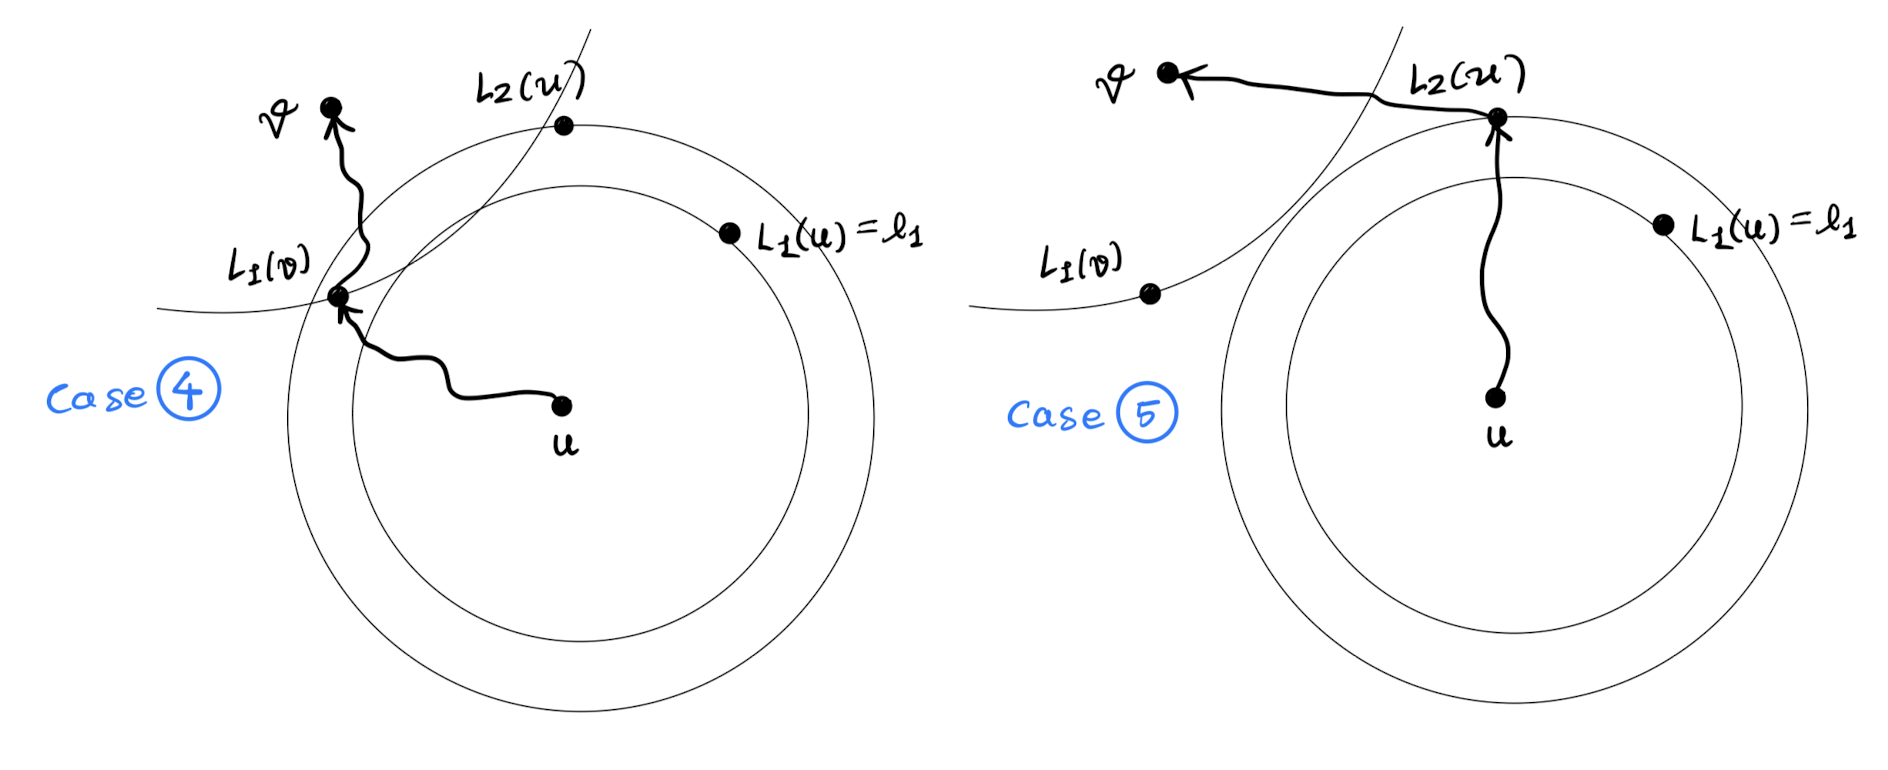
\includegraphics[width=0.8\textwidth]{img/correctstretch.png}
        \caption{Cases while generalising to 5-Approximate Distance Oracle}
        \label{fig:correctstretch}
    \end{center}
\end{figure}


\section{(2k-1)-Approximate Distance Oracle}

Building on our analysis of the 5-approximate distance oracle, we extend these ideas to construct a \((2k-1)\)-approximate distance oracle for any positive integer \(k\).

At each level, vertices are sampled with a specific probability, and local distance information is stored similarly to the 3-approximate case. The hierarchical structure allows us to bridge longer distances at higher levels, ensuring the overall approximation factor does not exceed \((2k-1)\).

This multi-level design preserves theoretical guarantees while improving both storage efficiency and query time for large graphs. In the following sections, we detail the construction of the oracle, explain the hierarchical sampling process, and analyze the algorithms for preprocessing, query answering, and their respective complexities.

\subsection{Construction of the \((2k-1)\)-Approximate Distance Oracle}

 The key insight is to always be able to jump from u. Further, we can exploit the symmetry of the distance calculation and conclude that the jump from the destination vertex also must be single. So, we would have to maintain balls of vertices from Landmarks of all levels for every vertex. Employing a hierarchical sampling scheme, we effectively will try to find an intermediate vertex in each of the balls to see if u or its focus belonging to the next level are in a common ball. We thus maintain localized distance information in a series of hash tables, which enables constant-time query answers. The construction proceeds as follows:

\begin{enumerate}
    \item \textbf{Hierarchical Sampling:} We maintain \( k \) ``levels'' of landmark vertice ``sets'' \{\( \text{landmark}^0, \\ \text{landmark}^1, \ldots, \text{landmark}^k \)\}, starting with \( \text{landmark}^0 = V \). For each \( 1 \le i \le k \), every vertex in \( \text{landmark}^{i-1} \) is included in \( \text{landmark}^i \) independently with probability \( n^{-1/k} \). Allowing vertices having a max level (called as the \emph{rank}, henceforth) allows us to handle cases ensuring that a focus of higher level is always the same or farther than the lower level.

    \item \textbf{Local Distance Storage:} We define the notion of locality using closest landmark at any level \textit{i}. For each vertex \( u \in \text{landmark}^i \), we define its \emph{focus set} at level \( i \) as
    \[
    \text{focus}_i(u) :=  v \,|\, v \in \text{landmark}^{i+1} \text{ and } \delta(v, u) \le \delta(u, w) \text{ for all } w \in \text{landmark}^{i+1} ,
    \]
    i.e., the closest landmark vertices at level \( i+1 \) to \( u \).\\
    Using this, we define the locality of vertex \textit{u} as \emph{ball} of \( u \) at level \( i \) as
    \[
    \text{Ball}_i(u) := \left\{ v \,\middle|\, v \in \text{landmark}^i \text{ and } \delta(v, u) \le \text{focal\_distance}_i(u) \right\},
    \]
    where \( \text{focal\_distance}_i(u) \) denotes the distance from \( u \) to its closest landmark in \( \text{landmark}^{i+1} \), called as the \emph{focus}. These sets are used to store local distances needed for efficient query resolution.

    \item \textbf{Global Distance Storage:} From the landmarks at level \textit{k}, store distance to 
    all vertices \textit{u} to handle queries of far-away point. To handle this efficiently, add all the vertices in \(landmark^k\) in balls of all vertices. This will also help in efficient retrieval using hashing of the ball. 
\end{enumerate}

The complete data structure for the oracle is the collection
\[
\{\text{Ball}_i(u) : u \in V,\; 0 \le i \le k\}.
\]

\subsection{Size Analysis of the \((2k-1)\)-Approximate Distance Oracle}

We now analyze the expected size of the \((2k-1)\)-approximate distance oracle.  In our hierarchical sampling, each vertex from the preceding level is chosen for the next level independently with probability 
\(
p = \frac{1}{\sqrt[k]{n}}.
\)

For a fixed vertex \(u\) and a given level \(i\), suppose we order the remaining vertices in \(V \setminus \{u\}\) by increasing distance from \(u\). A vertex appears in \(\text{Ball}_i(u)\) if none of the vertices preceding it in this order have been sampled into \(landmark^{(i+1)}\). Consequently, the expected number of vertices in \(\text{Ball}_i(u)\) is bounded by
\[
\mathbb{E}[|\text{Ball}_i(u)|] \le \sum_{j=1}^{n-1}(1-p)^{j-1} = O\Bigl(\frac{1}{p}\Bigr) = O\Bigl(n^{1/k}\Bigr).
\]

Since there are \(k\) levels, the total expected storage for vertex \(u\) is
\(
O\Bigl(k \cdot n^{1/k}\Bigr).
\)\\
Summing over all \(n\) vertices, the overall expected size of the oracle becomes
\(
O\Bigl(n \cdot k \cdot n^{1/k}\Bigr) = O\Bigl(k\, n^{1+1/k}\Bigr).
\)

Thus, the \((2k-1)\)-approximate distance oracle requires an expected space of \(O(k\, n^{1+1/k})\), confirming its efficiency in terms of storage.

\subsection{Query Answering Procedure}

To determine an approximate distance between any two vertices \(u\) and \(v\) using our \(k\)-level oracle, we exploit the hierarchical data structure built during preprocessing and symmetry as in case of 5-Approximate Distance Oracle. Each \(focus_i(u)\) is stored in the corresponding hash table for \(\text{Ball}_i(u)\), the distance \(\delta(u,focus_i(u))\) is readily available.

The query answering mechanism for \textit{u, v} operates as follows:

\begin{enumerate}
    
    \item Set the level counter \(i = 0\).
    \item \textit{x = u}
    \item \textbf{While \(x\) is not found in \(\text{Ball}_i(v)\):}  
    \begin{itemize}
        \item Increment the level \(i\) by 1.
        \item x = \(focus_i(u)\)
    \end{itemize}
    \item ans =
    \(
    \delta(u, x) + \delta(x, v),
    \)

    \item Set the level counter \(i = 0\).
    \item \textit{x = v}
    \item \textbf{While \(x\) is not found in \(\text{Ball}_i(u)\):}  
    \begin{itemize}
        \item Increment the level \(i\) by 1.
        \item x = \(focus_i(v)\)
    \end{itemize}
    \item ans =
    \(
    min(ans, \delta(u, x) + \delta(x, v)),
    \)
    
    which serves as the \((2k-1)\)-approximation of the true shortest path distance between \(u\) and \(v\).
\end{enumerate}

Since the search in each level involves a constant-time hash table lookup and the number of levels is bounded by \(k\), the query answering process requires at most \(k+1\) steps.  Consequently, the overall query time is \(O(k)\) in practice.

\subsection{Proof of Correctness}

We now show that the query algorithm always returns a distance that is within a factor of \((2k-1)\) of the true distance between any two vertices \(u\) and \(v\). The algorithm operates symmetrically for \(u\) and \(v\) and examining successive levels of our hierarchy which is a direct extension of our methodology for 5-Approximate Distance Oracle.

We argue by induction that after each iteration of the algorithm, the additional distance from the currently examined vertex to its chosen representative is bounded by 2 \(\delta(u,v)\). More concretely, let us denote by \(focus_{i+1}(u)\) the representative for the current vertex \(u\) at the \((i+1)\)th level. We claim that after \(i\) iterations, the distance from \(u\) to \(focus_{i+1}(u)\) is at most \(i \cdot \delta(u,v)\).

\textbf{Base Case (\(i=0\)):}  
Initially, we set \(x=u\), so the extra distance is
\(\delta(u,v) = 0\)
which is trivially within \(0 \cdot \delta(u,v)\).

\textbf{Inductive Step:}  
Assume that after \(j\) iterations, the distance from the current vertex to its representative is bounded by
\(
\delta(u, focus_{j+1}(u)) \le j\,\delta(u,v).
\)\\
Now, consider the \((j+1)\)th iteration. If the algorithm has not yet terminated, it implies that the  \(focus_{j+1}(u)\) is not sufficiently close—in particular, it does not belong to the corresponding ball of the other vertex. By the construction of the oracle, the new \(focus_{j+2}(u)\)
\[
\delta(v, focus_{j+2}(u)) \le \delta(v, focus_{j+1}(u)).
\]
Applying the triangle inequality, we have
\[
\delta(v, focus_{j+1}(u)) \le \delta(u,v) + d(u, focus_{j+1}(u)).
\]
From  inductive hypothesis \(\delta(u, focus_{j+1}(u)) \le j\,d(u,v)\), it follows that
\[
\delta(u, focus_{j+1}(u)) \le \delta(u,v) + j\,\delta(u,v) = (j+1)\delta(u,v).
\]
Therefore, the extra distance incurred in the \((j+1)\)th iteration is at most \((j+1)\delta(u,v)\), which completes the inductive step.

\textbf{Final Bound:}  
When the algorithm terminates at some iteration \(l\) (with \(l\le k\)), it reports the approximate distance as
\(
\delta_{\text{approx}}(u,v)=\delta(u, focus_l(u)) + \delta(v, focus_l(u)).
\)
From the inductive argument, we know that \(\delta(u, focus_l(u)) \le (l-1)\delta(u,v)\). Moreover, by the triangle inequality,
\[
\delta(v, focus_l(u)) \le \delta(u,v) + \delta(u, focus_l(u)) \le \delta(u,v) + (l-1)\delta(u,v).
\]
Thus,
\[
d_{\text{approx}}(u,v) \le 2(l-1)\delta(u,v) + \delta(u,v) = (2l-1)d(u,v).
\]
Since \(l\le k\), this guarantees that
\[
d_{\text{approx}}(u,v) \le (2k-1)\delta(u,v).
\]

This completes the proof that the algorithm provides a \((2k-1)\)-approximate distance between \(u\) and \(v\).\\
\textbf{Note:} Since, the loop may break at \(i \leq k\), we need not to go all the way upto k, thus giving shorter stretch than k in some cases. 

\subsection{Complexity for (2k-1)-Approximate Distance Oracles}

In this section, we describe a polynomial time algorithm for constructing a \((2k-1)\)-approximate distance oracle. The approach extends the earlier 3-approximate method via a hierarchical sampling strategy. After forming the sequence of sampled vertex sets, the remaining work consists of computing, for each vertex \(u\) and for each level \(i \le k\), the set \(\text{Ball}_i(u)\) along with the distances from \(u\) to vertices in these sets. The following subsections outline the key components of the construction and their analysis.
\\\\
\textbf{Focus of all vertices at all levels}
For every vertex \(u \in V\) and each level \(i\), we need to determine \(focus_i(u)\), the closest vertex in \(landmark^{(i+1)}\) to \(u\). A standard way to solve this is to augment the graph by adding a dummy vertex \(s\) connected via zero-weight edges to every vertex and then run Dijkstra's algorithm from \(s\). This procedure takes \(O(m \log n)\) time per level, and by processing all levels, we obtain an overall cost of \(O(k\,m \log n)\) for computing the representatives.
\\\\
\textbf{Efficient Computation of Balls}
\newline

For each vertex \(u\) and for each level \(i\) with \(1 \le i < k\), we define the set
\[
\text{Ball}_i(u) = \{v \in landmark^{(i)} \mid \delta(u,v) < \delta(u, focus_{i}(u))\}.
\]

To compute these sets efficiently for a vertex \textit{u}, we look for vertices \textit{v} such that \(u \in Ball_i(v)\) as the expected number of vertices \textit{v} is bounded. Thus, for any vertex \(v \in landmark^{(i)}\), define the group as follows:
\[
G_{i+1}(v) = \{w \in V \mid v \in Ball_i(w)\}.
\]
\\
\textbf{Trim Dijkstra’s Algorithm for Group Computation}\\

A key observation is the following lemma: \\
\textbf{Lemma: } On the shortest path from vertex \textit{u} to \(v \in G_i(v)\)  , all the vertices must also belong to \(G_i(v)\). \\

Using property that as Dijkstra progresses, the distance computed never increases, we need to visit only those vertices which belong to \(G_i(u)\) at any point in Dijkstra. This means, an edge (\textit{v}, \textit{y}) is relaxed using an addition condition from vertex \textit{v} which is:
\[
d(u, v) + \text{weight}(v, y) < \delta(y, L(y))
\]
This restriction ensures that vertices falling outside the group are not explored.

Since each edge relaxation using a min-heap takes \(O(\log n)\) time, the total time for computing a single group \(G_{i+1}(v)\) is proportional to the sum of the degrees of vertices in the group multiplied by \(\log n\). Summing over all group at a given level yields an overall cost of
\(
O\left(\sum_{u \in V} |\text{Ball}_i(u)| \log n\right).
\)
Given that the expected size of \(\text{Ball}_i(u)\) is \(O(n^{1/k})\), the expected cost for level \(i\) is \(O(m\,n^{1/k}\log n)\). By processing all \(k\) levels, the total cost for computing ball sets is \(O(k\,m\,n^{1/k}\log n)\). With Fibonacci heaps, one can reduce or eliminate the logarithmic factor.
\\\\
\textbf{Overall Running Time and Space Analysis}\\
Combining the time for sampling, computing focii, and forming the balls, the total expected running time for building the data structure is
\({O}(k\,m\,n^{1/k}),
\).

Concerning space, each level \(i\) contributes an expected \(O(n^{1/k})\) elements per vertex, resulting in an overall expected space usage of
\(
O\left(n \cdot k \cdot n^{1/k}\right) = O\Bigl(k\,n^{1+1/k}\Bigr).
\)
To guarantee a worst-case size of \(O\Bigl(k\,n^{1+1/k}\Bigr)\) for the data structure, we rerun the entire preprocessing algorithm. Since the expected number of repetitions required to achieve this bound remains constant, the overall asymptotic performance is not adversely affected.

\subsection{Final Result}
We thus conclude that, for a weighted undirected graph \(G=(V,E)\) and an integer \(k\), one can build a data structure of expected size \(O\Bigl(k\,n^{1+1/k}\Bigr)\) in \(O\bigl(k\,m\,n^{1/k}\bigr)\) time. This data structure enables us to report a \((2k-1)\)-approximate distance between any two vertices in \(O(k)\) time.

\section{Implementation Details}

C++ was chosen as the language for experimentation as it provided greater control over memory allocation and internal data structures. A visualization module was also created, based on initial prototyping in Python, for additional support. All charts were generated using Python and Jupyter Notebooks. Each directory includes a \texttt{README} file containing exact instructions on how to run and use the code.

\subsection*{Key Implementation Details}

\begin{enumerate}
    \item Initially, we started with a simple modular implementation of the code. However, for larger graph sizes (around 1000 nodes), memory pressure became significant due to edge weights being of type \texttt{double} (8 bytes). Consequently, the codebase was restructured into two separate executables with an object-oriented design.
    
    \item STL-based containers were primarily used, as they provided robust and efficient performance for our use case.
    
    \item To test various edge cases, we added support for custom landmark selection.
    
    \item For computing true distances between vertices, two methods were implemented: one using the Floyd-Warshall algorithm and the other using Dijkstra's algorithm for each query.
    
    \item A Python script was created to generate queries, either exhaustively or by uniformly sampling the required number of queries.
    
    \item Since the default \texttt{unordered\_map} in STL does not guarantee worst-case constant-time lookup, we opted for an alternative implementation using the FPH library~\cite{fphlib}. Hashing was performed using the FCH algorithm with a \texttt{MixSeedHash} function, as part of the \texttt{metaFPHMap} table, resulting in very low output query time.
\end{enumerate}

\subsection*{Choice of Datasets}

\begin{enumerate}
    \item We explored various publicly available datasets and made the following observations:
    \begin{itemize}
        \item Most real-world datasets were unweighted.
        \item They were either too small (a few KBs to MBs) or too large (around 10GB).
        \item Many datasets were unclean, containing inconsistencies such as duplicate edges, incorrect metadata (e.g., number of nodes), and format anomalies. Cleaning these required significant manual preprocessing.
    \end{itemize}
    Therefore, we selected representative graphs from three categories:
    \begin{enumerate}
        \item RoadNet California~\cite{roadnet}
        \item Facebook Social Circles~\cite{facebook}
        \item Enron Email Cluster and Hierarchical Structure~\cite{enron}
    \end{enumerate}

    \item To address the limitations of real-world datasets, we generated synthetic graphs to obtain fine-grained control over parameters such as average degree and number of nodes.

    \item We attempted to run our algorithm on large datasets (around 10GB) on CSE servers, but due to memory usage exceeding 90GB and long runtimes (5--6 hours), we restricted ourselves to graphs with up to 50,000 nodes.

    \item Approximately 30 runs were conducted on different graph datasets. A summary of the results is provided in the following section.
\end{enumerate}

\subsection*{Key Observations}

\begin{enumerate}
    \item For a fixed $k$ and average degree, as $n$ increases, the stretch distribution shifts to the right; however, the frequency of stretch values close to 1 remains high.

    \item The use of the custom hashing function maintained an average query time of approximately 400ns, with minimal variation as $k$ increased.

    \item The number of words used to represent graphs was exponentially smaller than the $O(n^2)$ worst-case expectation across all test cases.

    \item As the average degree decreased, instances of higher stretch became more frequent.

    \item For graphs with more than 1000 nodes, the overall stretch remained consistently low.
\end{enumerate}

\begin{figure}
\begin{center}
    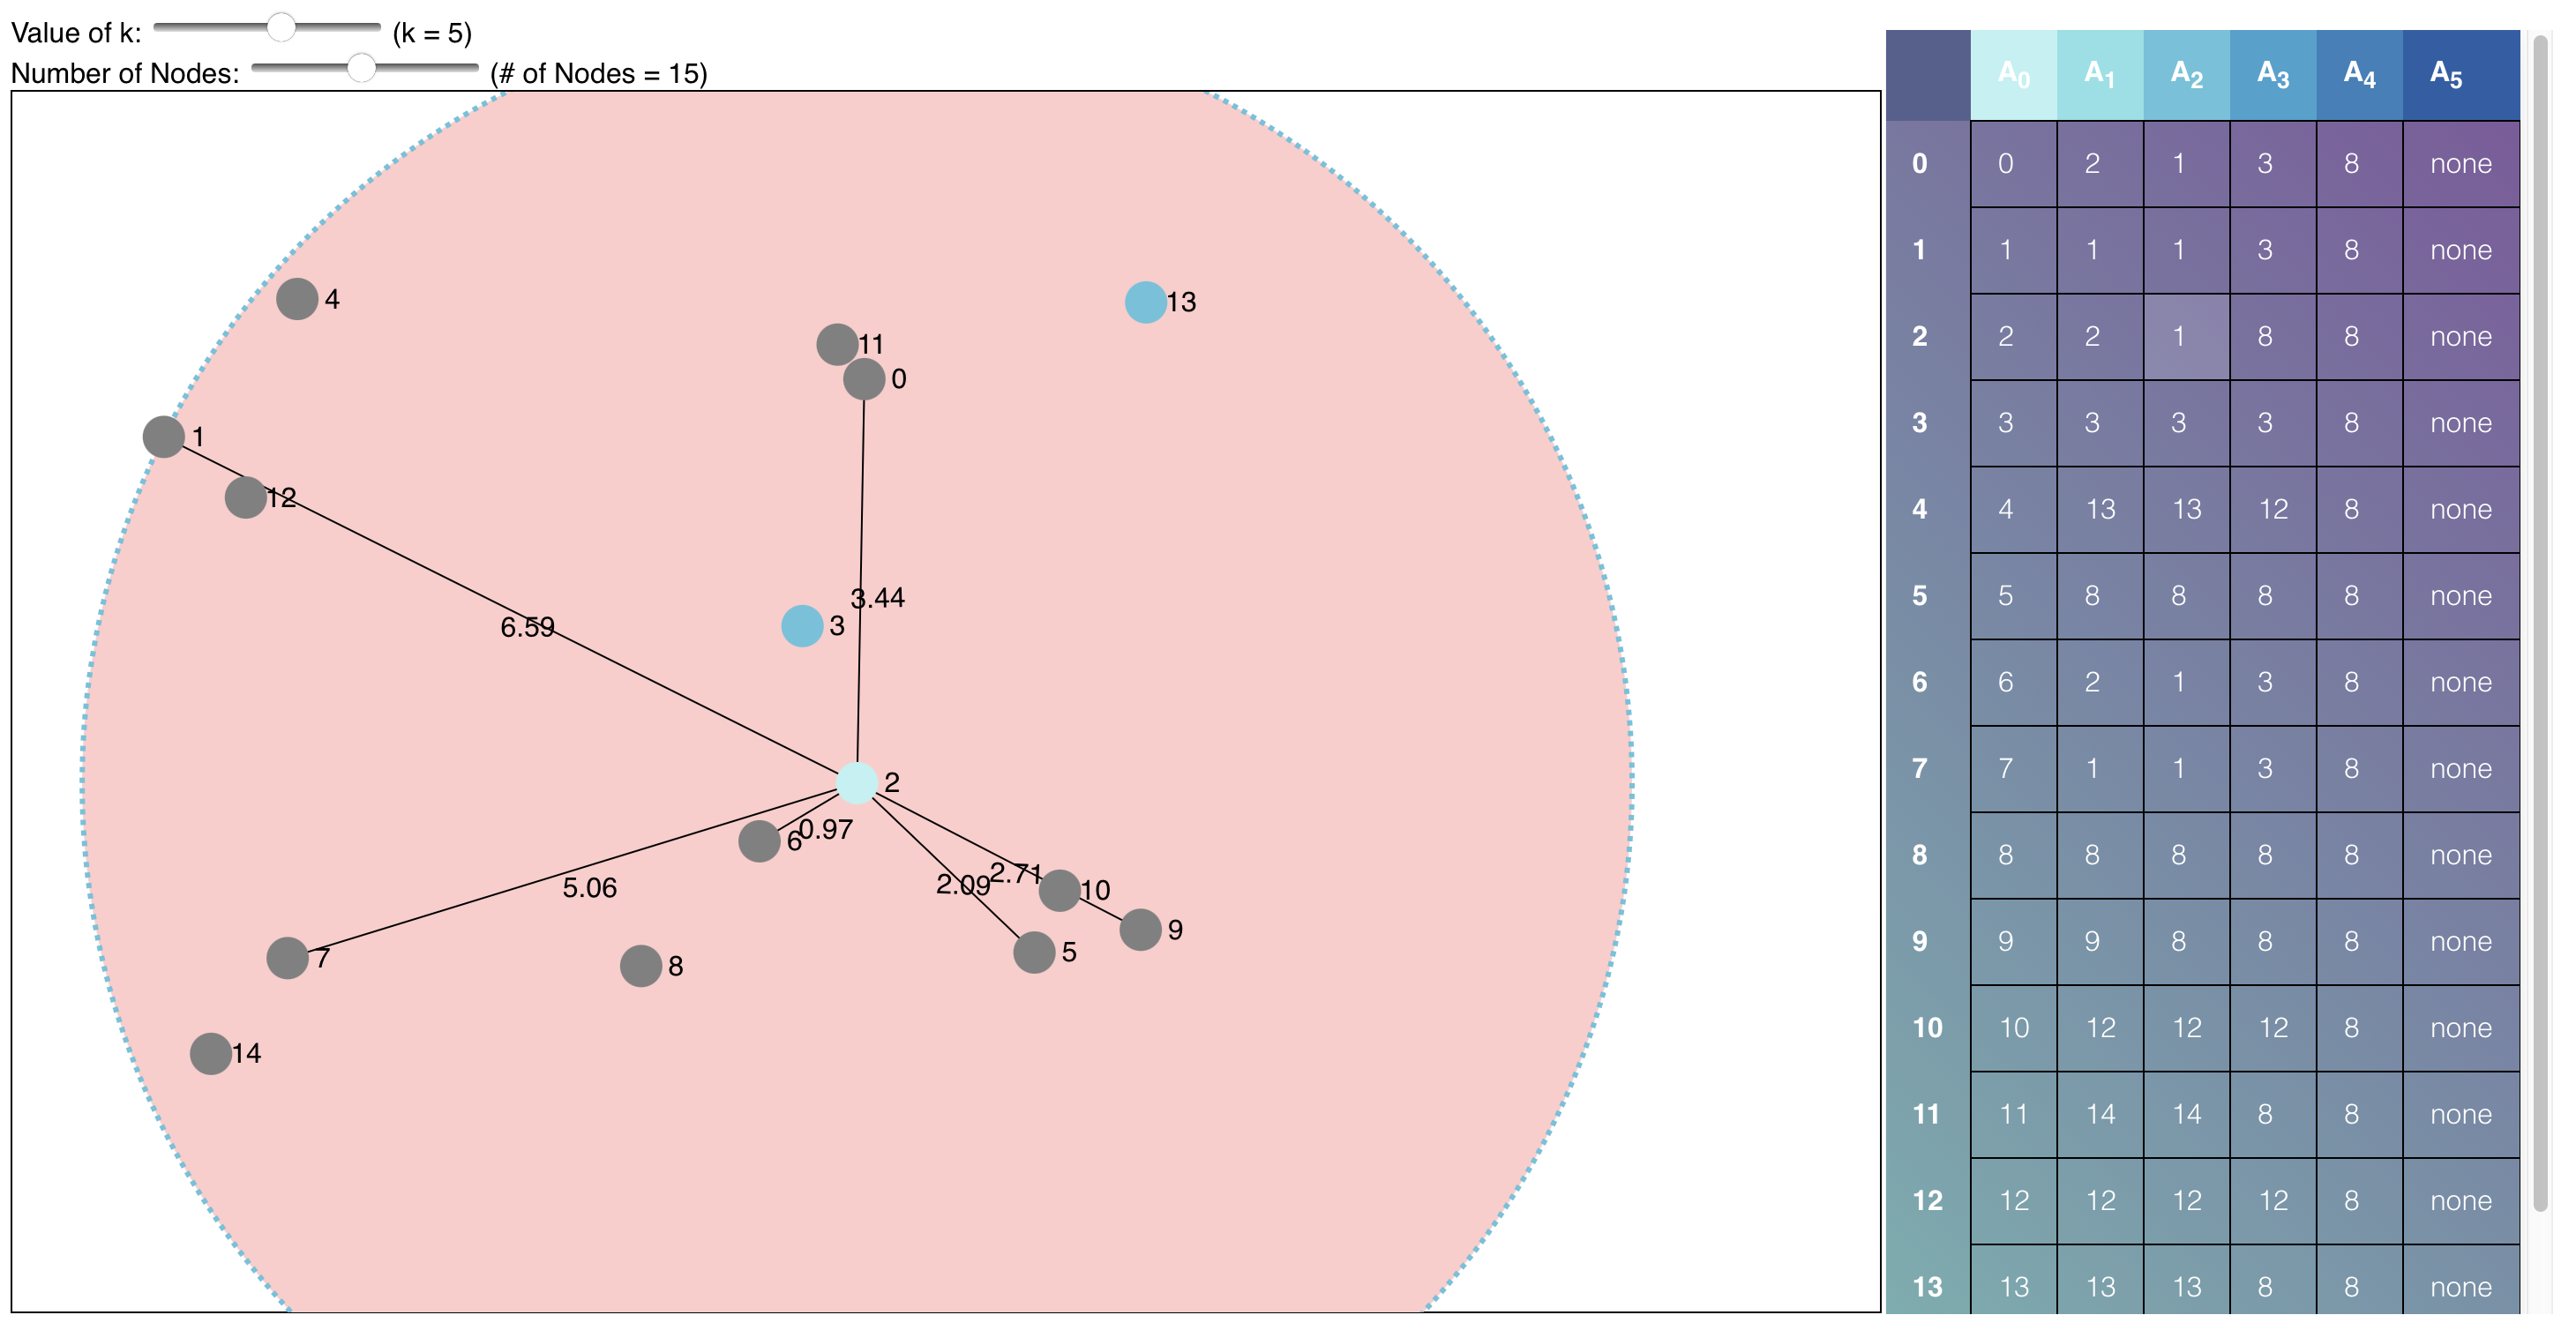
\includegraphics[width=0.9\textwidth]{img/v1.png}
    \caption{Visualisation}
    \label{fig:visualisation1}
\end{center}
\end{figure}

\begin{figure}
\begin{center}
    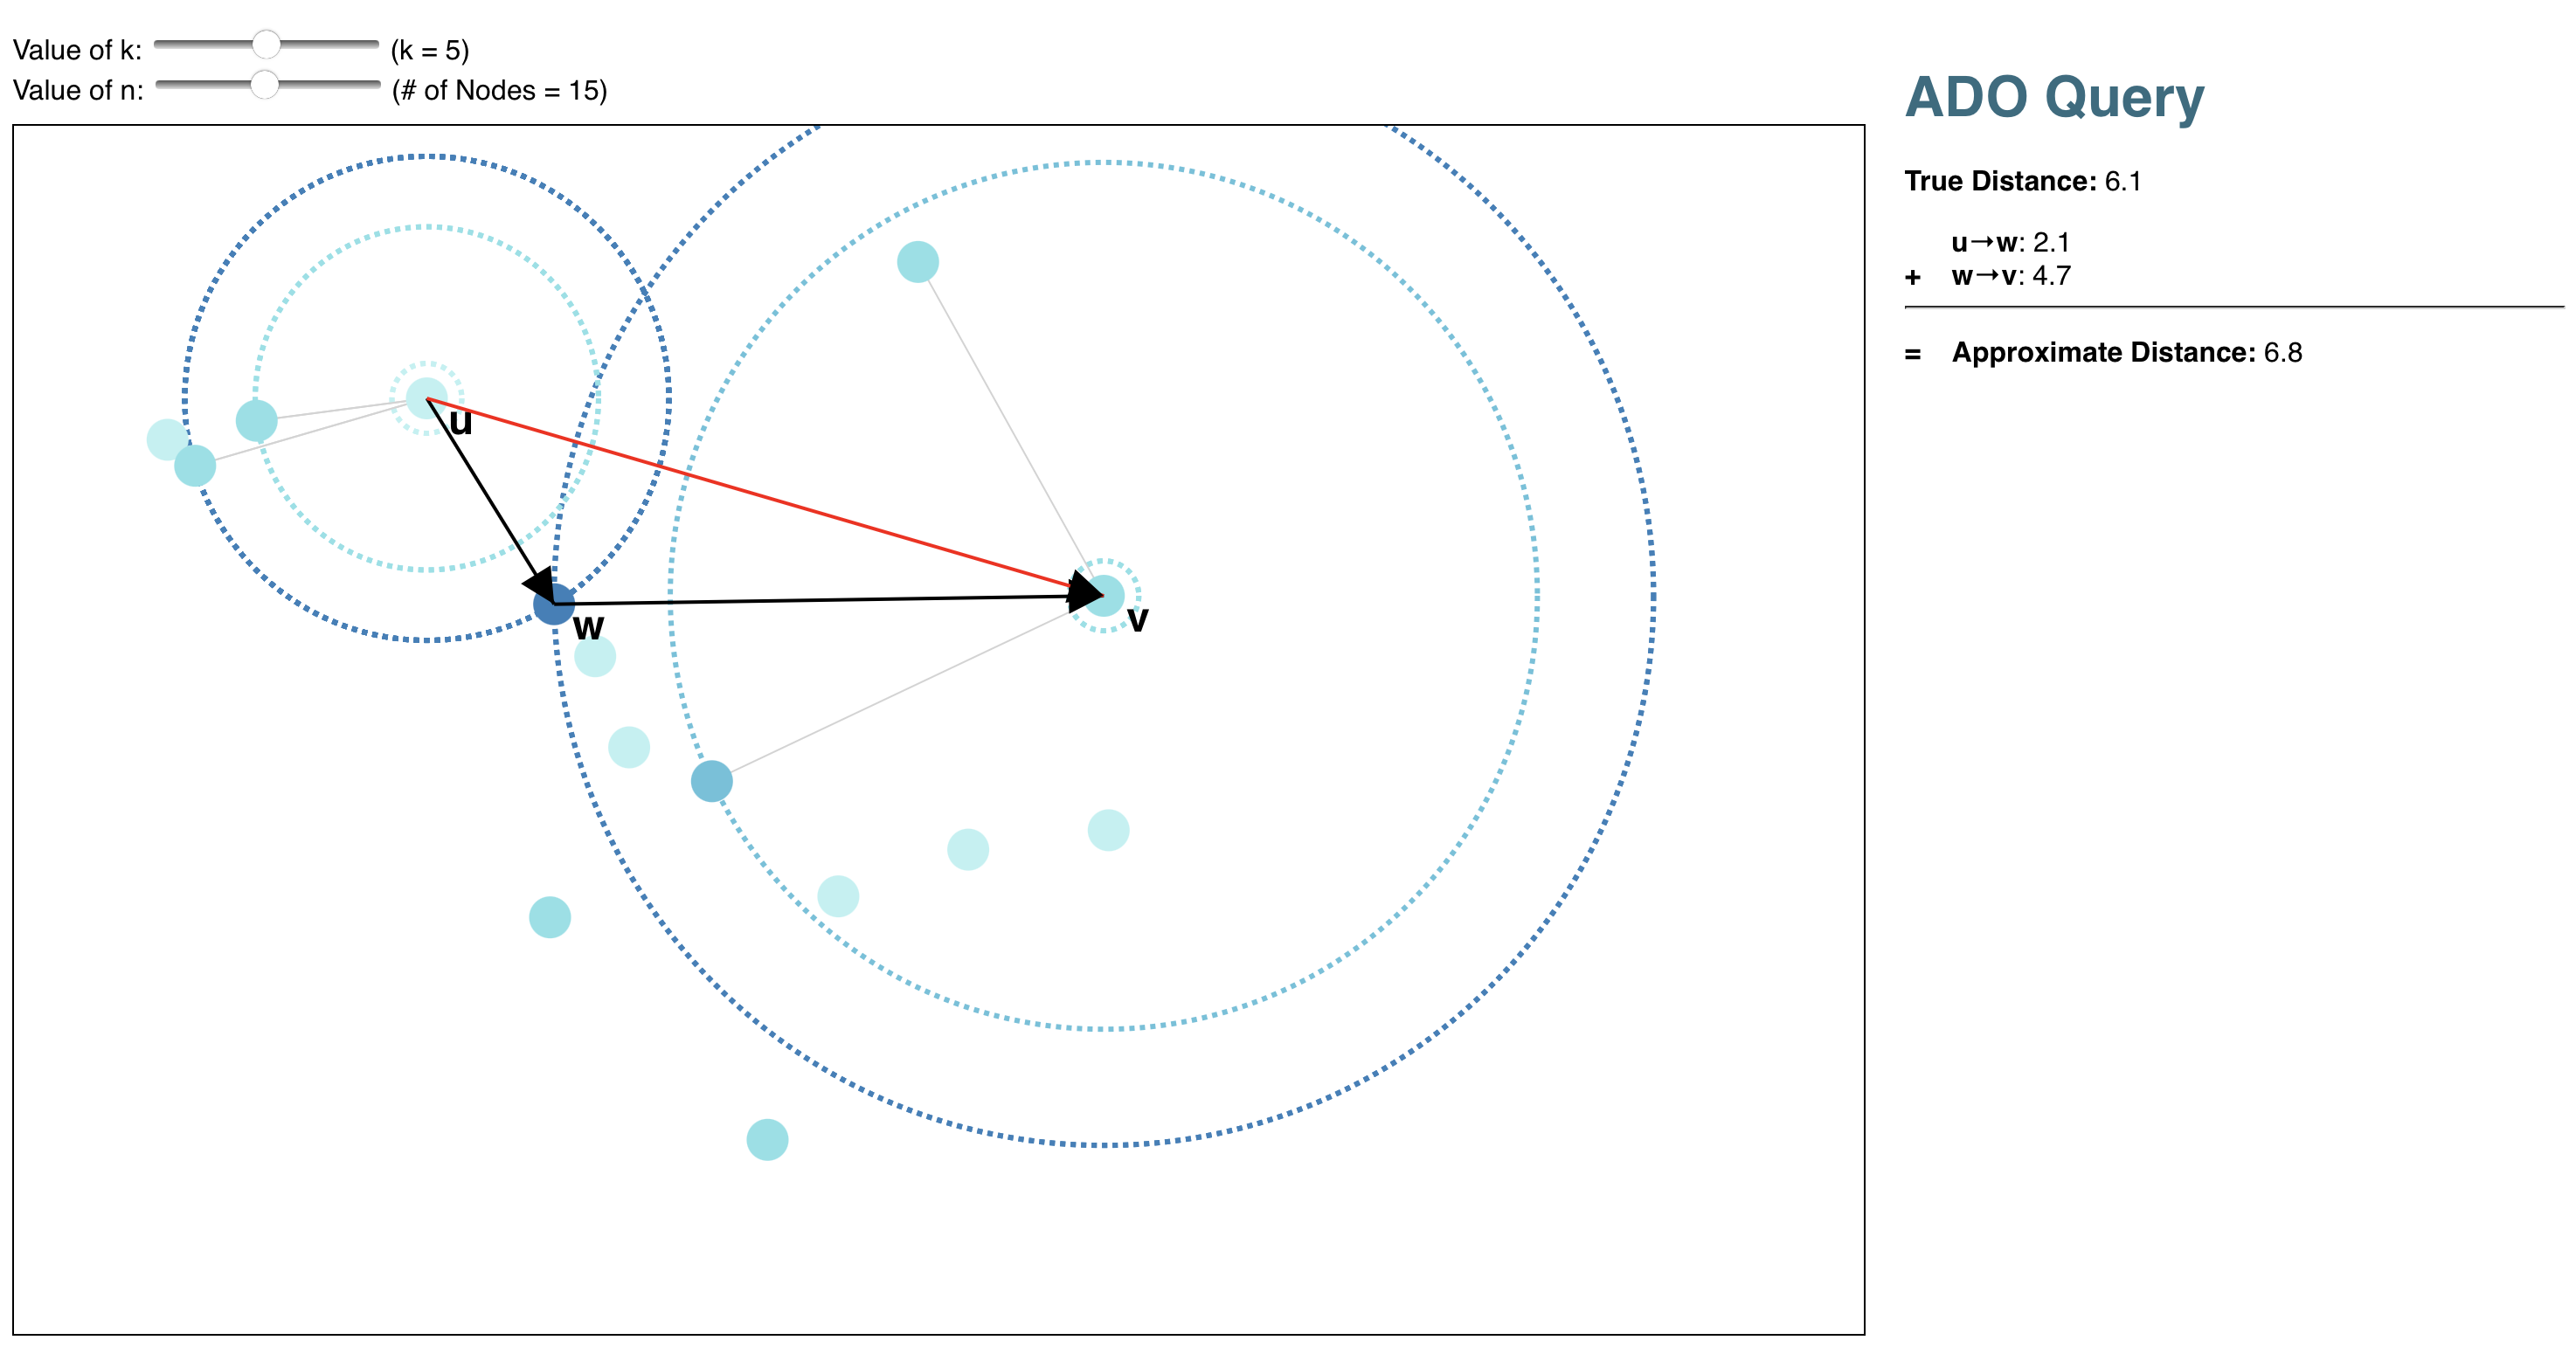
\includegraphics[width=0.9\textwidth]{img/v2.png}
    \caption{Visualisation}
    \label{fig:visualisation2}
\end{center}
\end{figure}

\section{Future Work}

\begin{itemize}
    \item \textbf{Parallelization for Fast Pre-Processing:} One promising direction is to parallelize the preprocessing phase. Since computing local distance information and forming the clusters or ball sets for each vertex can be done independently, distributing this work across multiple processors or cores can significantly reduce the overall runtime.
    
    \item \textbf{Dynamic Updates:} Enhancing the data structure to support dynamic updates—such as insertions, deletions, or weight modifications—without requiring a full re-preprocessing of the graph would make the oracle more practical for real-time or evolving networks.
\end{itemize}

\begin{thebibliography}{9}
    \bibitem{fphlib} \url{https://github.com/renzibei/fph-table/tree/master}
    \bibitem{roadnet} \url{https://snap.stanford.edu/data/roadNet-CA.html}
    \bibitem{facebook} \url{https://snap.stanford.edu/data/ego-Facebook.html}
    \bibitem{enron} \url{https://snap.stanford.edu/data/email-Enron.html}
    \end{thebibliography}

\end{document}
